\section{Problemanalyse \label{sec:problemanalyse}}
Problemanalysen tager udgangspunkt i nøgleproblemet spildtid jf. projektbeskrivelsen i appendikssektionen (\ref{appendix:projektbeskrivelse}). 


\subsection{Problemtræ}
Forneden har vi fremstillet et problemtræ, der viser nogle af årsagerne til tidsspild og nogle af virkningerne.
\begin{figure}[H]
    \centering
    \resizebox{\columnwidth}{!}{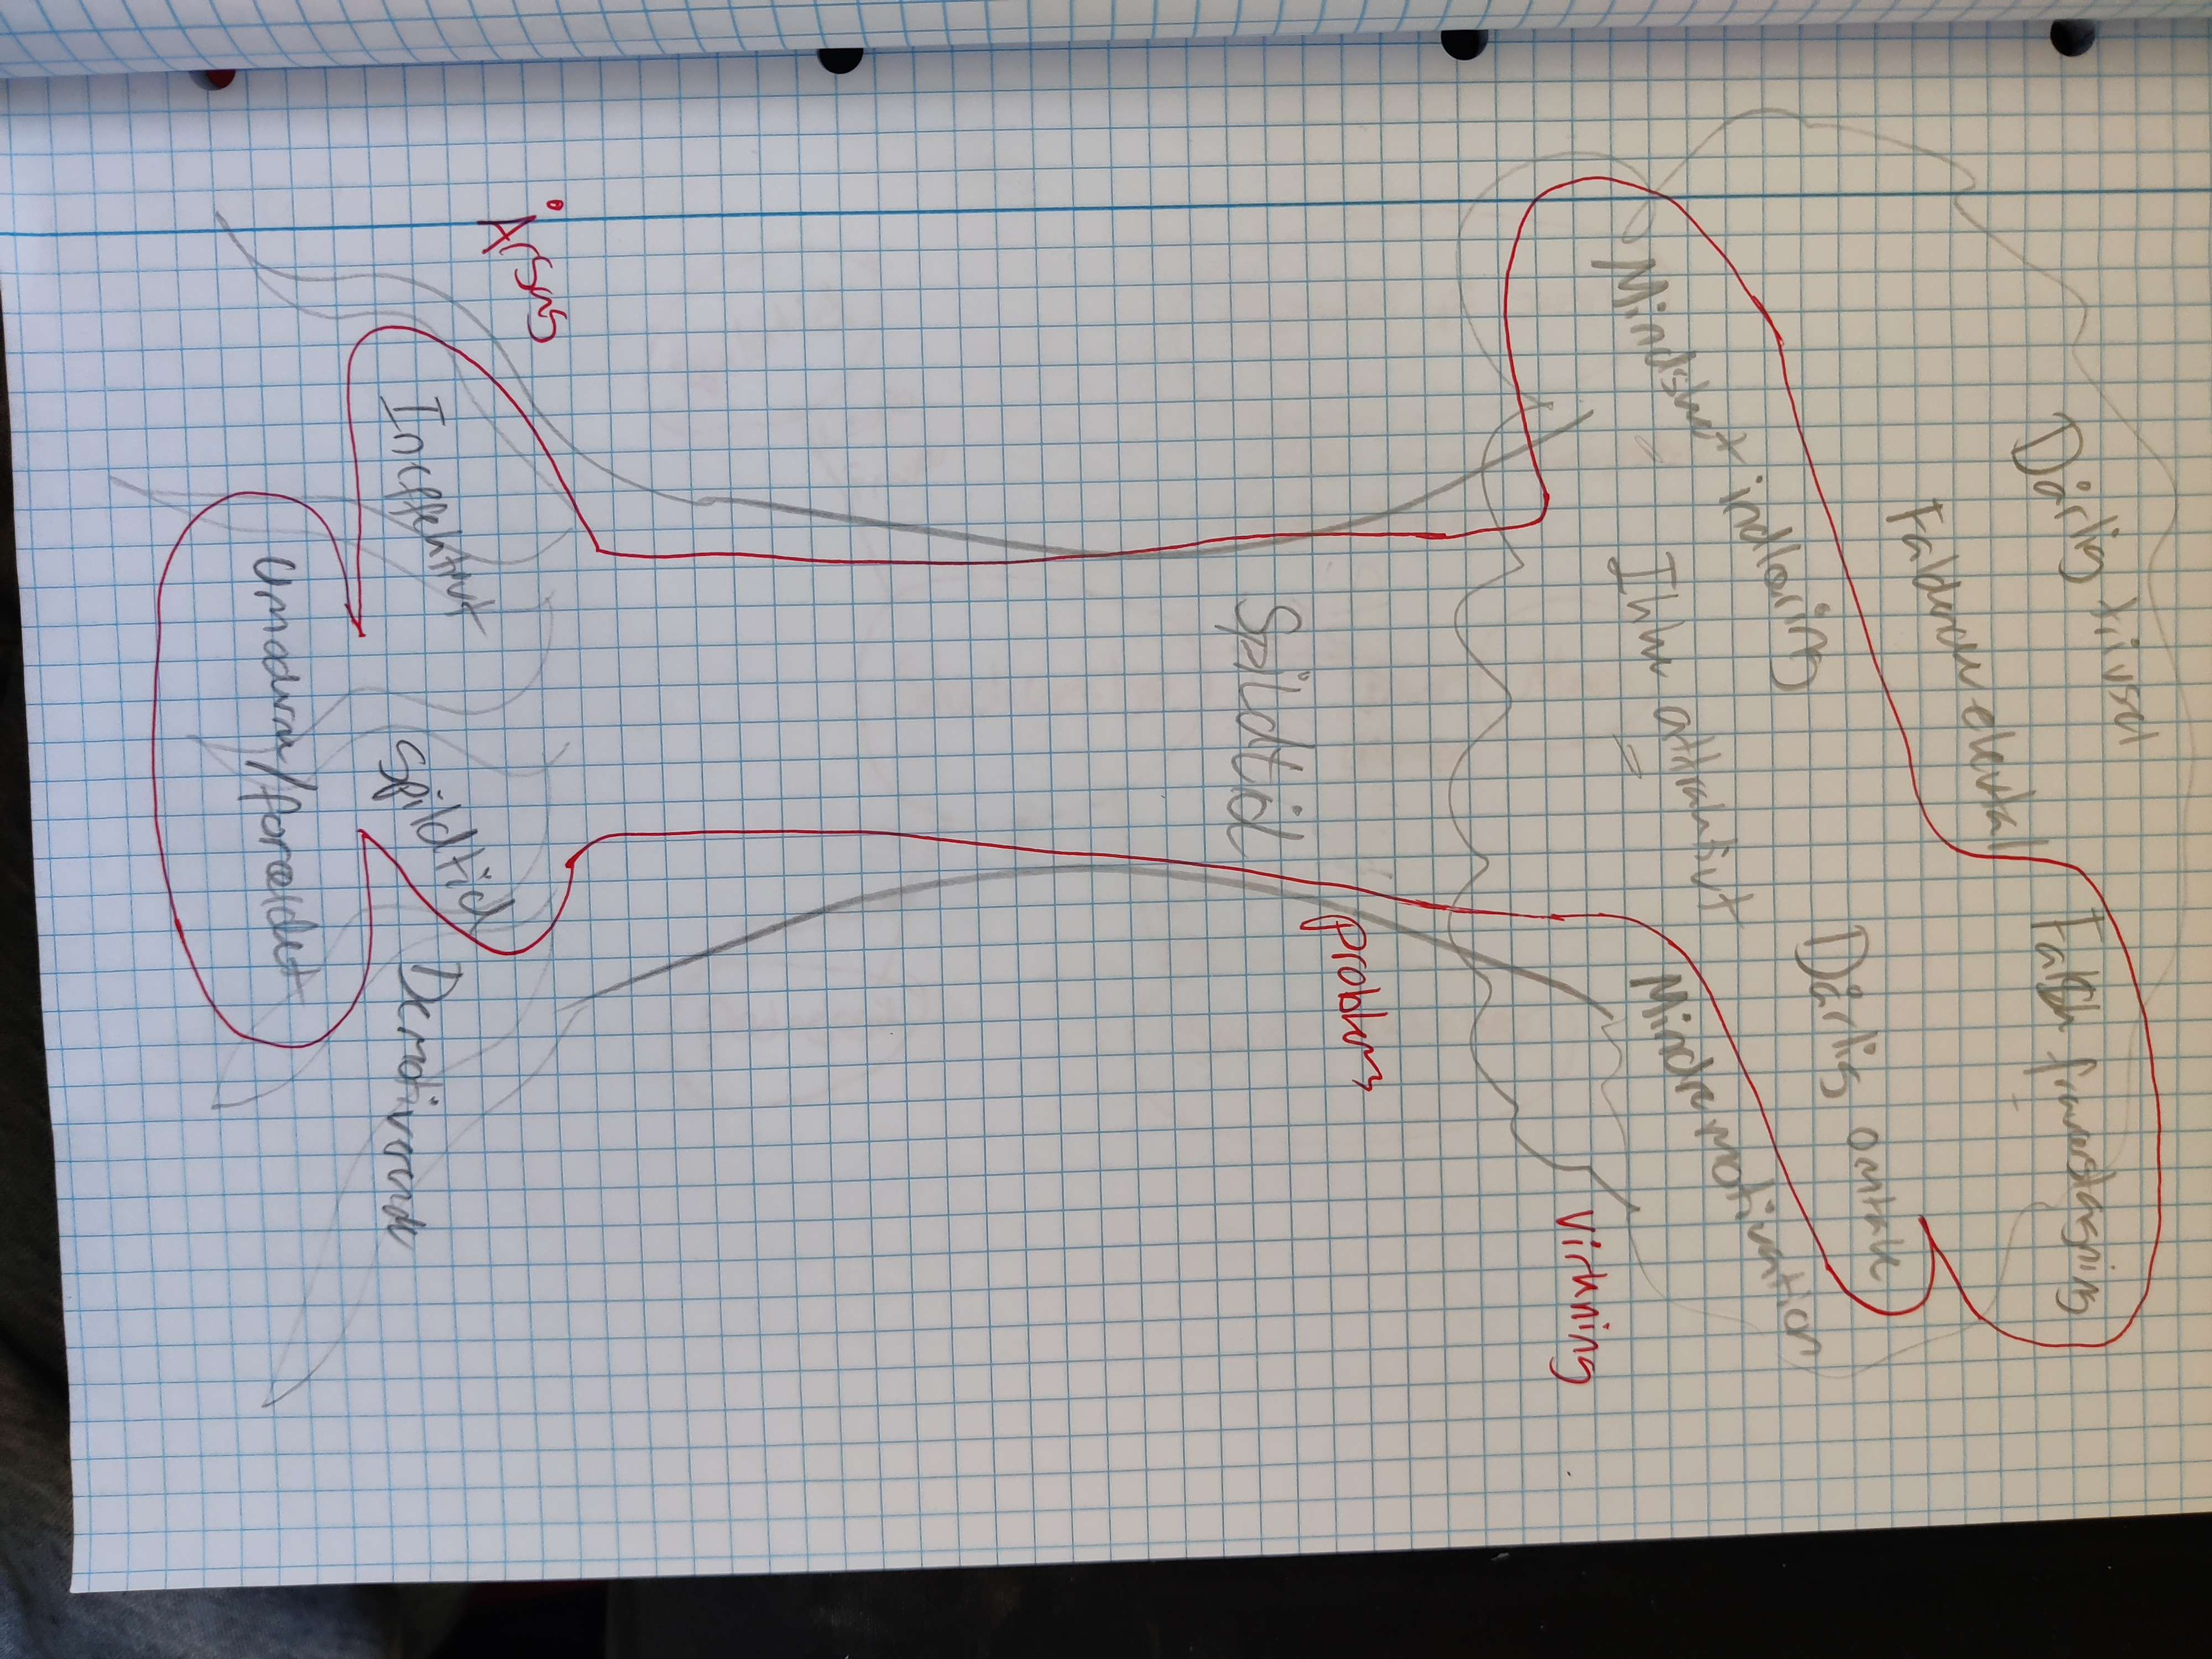
\includegraphics[angle =90]{assets/problemtrae.jpg}}
    \caption{Viser problemtræet, der blev anvendt i problemanalysen.}
\end{figure}
Et af de ineffektive systemer, vi kom i tanke om, er Lectio-applikationen, hvorefter vi har informationssøgt om emnet. Det var ikke muligt at finde nogle reele artikler om tidssplid med Lectio-applikationen, 
Da har vi forhørt os kvalitativt og snakket med flere medstuderende og flere underviserer (interessenter) som benytter sig at Lectio i deres dagligdag.
\subsection{Kvalitativ metode}
Forneden er vores overordnet indtryk af, hvordan de folk, vi har snakket med, opfatter lectio:
De har alle udtalt sig om Lectios unødvændigt komplicerede designvalg, forældede udseende og mangler. Vi snakkede bl.a. Med en underviser som udtrykte sin fustrattion over 
at det nuværende Lectio kun kan uploade et dokument ad gangen. Dette fandt vi meget mærkeligt, da vi har en udvidet viden om webudvikling, og ergo ved vi at sådan en funktion (multiupload) er utrolig nem at 
implementere og stod tilbage uforstående for, at Lectio ikke havde mulighed for så basal funktionalitet som det. Det kan også hurtigt tage fx. 10 sekunder at navigere hen til en fil og derefter uploade den, så hvis man vil uploade fx. >>20 filer<<, så tager dette altså 200 sekunder tilsvarende til 3 minut og 20 sekunder. 

\subsection{HV-modellen}
Herefter er HV-modellen i sammenspil med den kvalitative undersøgelse i forrige kapitel, blevet anvendt til at få en ide om handlingsplanen, forbrugernes mangler og dermed potentielle produktbehov:
\paragraph{Hvad?}
    Det man skal gøre er altså at implementere basale QOL-features (Quality-of-life; rare features at have) ved at lave et rework af Lectio. På nuværende tidspunkt er vi ikke klar over, hvem der maintainer Lectio-applikationen, ej heller hvilke tiltag de gør for at modernisere denne.
\paragraph{Hvorfor?}
    Det skal gøres, så man i fremtiden kan spare tid og tankekraft ved at gøre Lectio til en bedre IT-løsning; et system, der gør det attraktivt at anvende til at centralisere informationsdeling, således at brugere ikke søger afsides og udliciterer opgaven til 700 andre tjenester samt gør det nemtoverskueligt for brugeren at orientere sig; hvilket gør at læringen kan komme i fokus, fremfor IT-stads. 
\paragraph{Hvem?}
    Hvem bør gør det? Det er selvfølgelig Lectio
\paragraph{Hvordan?}
    De bør gøre det ved at anvende moderne webaplikkationsbyggeteknik; ændre deres techstack og designfilosofi.

\subsection{Envidere kritik af Lectios designfilosofi}
    Alle knapperne er små, og der er for mange af dem, det er for komplekst og der er meget redundans; mange måder, hvorpå man kan opnå samme resultater. 
    Farvevalget er også grimt; det ser visuelt forældet ud, hvilket ikke just inspirerer en gejst host kunden.
    Endvidere kan Lectio overhovedet ikke scalerer, altså når man ændre skærmstørelsen forbliver Lectio samme størelse. Dette er et red flag for hjemmesider da korrekt websidedesignfilosofi
    siger at hjemmesider skal være responsive.

\subsection{Problemformulering \label{sec:problemformulering}}
    Det er et problem, at Lectios website er forældet, da dette resulterer i, at den ikke effektivt kan overlevere information til sine forbrugere, ej heller overskueligt intergeres med jf. problemanalysen (\ref{sec:problemanalyse}), hvorfor den ikke er berettiget i sin eksistens jf. Lectios eget informationsark, hvor de eksplicit udpenslerer dette som Lectios bærende hovedformål\cite{lectioark}.